%%%%%%%%%%%%%%%%%%%%%%
\documentclass{doublecol-new}
%%%%%%%%%%%%%%%%%%%%%%

\usepackage{natbib,stfloats}
\usepackage{mathrsfs}
\usepackage{graphicx}
\usepackage[labelsep=quad,font=small,justification=justified,singlelinecheck=false,format=plain,labelfont=bf,up,textfont=normal,up]{caption}
\usepackage{tabularx}
\usepackage{booktabs}
\usepackage{tabu}
\usepackage{listings}
\usepackage[table]{xcolor}
\usepackage[tableposition=top]{caption}
\usepackage{multirow}
\renewcommand{\lstlistingname}{Figure}
\renewcommand{\figurename}{Figure}

\makeatletter
\AtBeginDocument{%
  \let\c@figure\c@lstlisting
  \let\thefigure\thelstlisting
  \let\ftype@lstlisting\ftype@figure % give the floats the same precedence
}
\makeatother

\def\newblock{\hskip .11em plus .33em minus .07em}

\theoremstyle{TH}{
\newtheorem{lemma}{Lemma}
\newtheorem{theorem}[lemma]{Theorem}
\newtheorem{corrolary}[lemma]{Corrolary}
\newtheorem{conjecture}[lemma]{Conjecture}
\newtheorem{proposition}[lemma]{Proposition}
\newtheorem{claim}[lemma]{Claim}
\newtheorem{stheorem}[lemma]{Wrong Theorem}
\newtheorem{algorithm}{Algorithm}
}

\theoremstyle{THrm}{
\newtheorem{definition}{Definition}[section]
\newtheorem{question}{Question}[section]
\newtheorem{remark}{Remark}
\newtheorem{scheme}{Scheme}
}

\theoremstyle{THhit}{
\newtheorem{case}{Case}[section]
}

\makeatletter
\def\theequation{\arabic{equation}}

\JOURNALNAME{\TEN{\it International Journal of Embedded Systems,
Vol. \theVOL, No. \theISSUE, \thePUBYEAR\hfill\thepage}
}

%
%
%\def\BottomCatch{%
%\vskip -10pt
%\thispagestyle{empty}%
%\begin{table}[b]%
%\NINE\begin{tabular*}{\textwidth}{@{\extracolsep{\fill}}lcr@{}}%
%\\[-12pt]
%Copyright \copyright\ 2012 Inderscience Enterprises Ltd. & &%
%\end{tabular*}%
%\vskip -30pt%
%%%\vskip -35pt%
%\end{table}%
%}

\makeatother

%%%%%%%%%%%%%%%%%
\begin{document}%
%%%%%%%%%%%%%%%%%

\lstset{language=C,basicstyle=\small}
\lstset{numbers=left, numberstyle=\tiny, stepnumber=1, numbersep=5pt}
\lstset{tabsize=2}
\lstset{firstnumber=1}
\lstset{frame=single}
\lstset{
  language={C},
  morekeywords={assert,uchar}
}

\setcounter{page}{1}

%\LRH{A. Trindade et~al.}

\RRH{Multi-Core Model Checking and Maximum Satisfiability Applied to Hardware-Software Partitioning}

\VOL{x}

\ISSUE{x}

\PUBYEAR{xxxx}

\BottomCatch

%\CLline

\PUBYEAR{2012}

\subtitle{}

\title{Multi-Core Model Checking and Maximum Satisfiability Applied to Hardware-Software Partitioning}

\authorA{Author A}
\affA{University A\\
E-mail: \{nonono\}@nonono.com}

\authorB{Author B}
\affB{University B\\
E-mail: \{nonono\}@nonono.com}


%\authorA{Alessandro Trindade, Hussama Ismail}
%\affA{Federal University of Amazonas \\
%E-mail: \{alessandro.b.trindade, hussamaismail\}@gmail.com}

%\authorB{Edilson Galv\~ao, Renato Degelo}
%\affB{Federal University of Amazonas \\
%E-mail: \{rdegelo, esj.galvao\}@gmail.com}

%\authorC{Helder Silva, and Lucas Cordeiro}
%\affC{Federal University of Amazonas \\
%E-mail: prhsilva2012@gmail.com, lucascordeiro@ufam.edu.br}

\begin{abstract}
We present new alternative approaches to solve the hardware and software (HW-SW) partitioning problem. First, we use Bounded Model Checking (BMC) based on Satisfiability Modulo Theories (SMT) in conjunction with a multi-core support using Open Multi-Processing to create four variants to solve the partitioning problem. Multi-core SMT-based BMC approach allows initializing many verification instances using different approaches based on the number of available processing cores. In particular, each instance checks for a different optimum value until the optimization problem is satisfied. We implement our algorithms on top of the Efficient SMT-Based Context-Bounded Model Checker (ESBMC). Additionally, we integrate the maximum satisfiability solver $\nu$Z tool into ESBMC, which provides a portfolio of approaches for solving linear optimization problems over SMT formulas. We compare all proposed approaches to a state-of-the-art optimization tool (MATLAB). Experimental results show that there is no single optimization tool to solve all HW-SW partitioning benchmarks.
\end{abstract}

\KEYWORD{hardware-software co-design, hardware-software partitioning, optimization, model checking, multi-core, maximum satisfiability.}

\REF{\textcolor{red}{to this paper should be made as follows: No no no. `Multi-Core Model Checking and Maximum Satisfiability Applied to Hardware-Software Partitioning', {\it International Journal of Embedded Systems}, Vol. x, No. x, pp.xxx\textendash xxx.}}

%Trindade, A., Ismail, H., Galv\~ao, E., Degelo, R., Silva, H., and Cordeiro, L.%
\begin{bio}
\textcolor{red}{
no no no.\vs{9}}

\textcolor{red}{\noindent No no no.\vs{8}}

\textcolor{red}{\noindent No no no.}
\end{bio}

\maketitle
\clearpage

\section{Introduction}

Nowadays, with the strong development of embedded systems, the design phase plays an important role. At early stages, the design is split into separated flows: hardware (HW) and software (SW). The partitioning decision process, which deals with decisions upon which parts of the application have to be designed in hardware and which one in software, must be supported by any well-structured methodology. If there is no methodology support, a number of issues, {\it e.g.}, design flow interruptions, redesigns, and undesired iterations may affect the overall development process, the quality, and the life-cycle of the final system.

Starting at the $90$'s decade, intensive research was performed in HW-SW partitioning, and several approaches proposed, as shown in~\cite{Arato2003} and~\cite{Mann2007}. In~\cite{Trindade2015} and~\cite{Trindade2016} was shown that it is possible to use Bounded Model Checking (BMC) based on Satisfiability Modulo Theories (SMT), implemented in a tool called Efficient SMT-Based Context-Bounded Model Checker (ESBMC) as defined in~\cite{Cordeiro2012}, in order to perform HW-SW partitioning in embedded systems. In~\cite{Trindade2016}, the original ESBMC algorithm was improved in terms of performance, so a multi-core sequential approach was introduced, in order to speed up the performance and turn it similar, in some cases, to conventional optimization tools, which are used to perform HW-SW partitioning.

The present work thus extends those previous studies since there is a substantial improvement in terms of the SMT-based verification methods. In particular, we extend the work of~\cite{Trindade2015} and~\cite{Trindade2016} to exploit a multi-core parallel- and binary-search approaches, as well as, the integration of the Maximum SMT (MaxSMT) solver $\nu$Z into ESBMC, which is a state-of-art optimization tool based on SMT as defined in~\cite{Bjorner2015}.

We exploit the availability of multi-core processors and the tool OpenMP as defined in~\cite{Tang2009}; thus, we apply SMT-based verification methods to the HW-SW partition problem in three different ways using a multi-core ESBMC approach with OpenMP: ESBMC-SS using a sequential-search (SS), ESBMC-PS using a parallel-search (PS), and ESBMC-PB using a binary-search (BS). Experimental results are compared to ILP (integer linear programming), GA (generic algorithms) in a multi-core version, and also to $\nu$Z, which supports only a single-core approach, according to~\cite{Bjorner2015}. The ILP and GA algorithms are implemented with the optimization toolbox of Matlab, according to~\cite{TheMathWorks2013}, while $\nu$Z is a built-in tool to the SMT solver Z3. All multi-core ESBMC approaches, together with $\nu$Z, are implemented with the ESBMC tool.

\subsection{Contributions} 

The main contribution of the present study is to describe and evaluate a comprehensive SMT-based BMC approach in a multi-core architecture applied to solve HW-SW optimization problems. Additionally, we integrate the MaxSMT solver $\nu$Z into an off-the-shelf BMC tool, which is typically used for software verification, in order to formulate and solve optimization problems within the logical context of constraints. Experimental results show that multi-core model-checking techniques can be effective, in particular cases, to find the optimal solution of the HW-SW partitioning problem using an SMT-based BMC approach. Although there is no single tool for efficiently solving all HW-SW partitioning problems, we show that the MaxSMT solver $\nu$Z is faster than other state-of-the-art optimization tools for small- and medium-size optimization problems.  To the best of our knowledge, this is the first work to use a multi-core SMT-based verification and a MaxSMT solver to check for HW-SW partitioning problems in embedded systems.

\subsection{Availability of Data and Tools}

Our experiments are based on a set of publicly available benchmarks. All benchmarks, tools, and results of our evaluation are available on a supplementary web page \texttt{http://esbmc.org/}.

\subsection{Organization of this Work}

This article is organized as follows: Section~\ref{background} gives a background on optimization techniques, $\nu$Z, ESBMC, and OpenMP tools. 
Section~\ref{Mathematical-modeling} describes the informal and formal mathematical modeling. The SMT-based BMC method is presented in Section~\ref{Analysis-of-the-partitioning-problem-using-ESBMC}, and in particular, Section~\ref{Analysis-of-the-partitioning-problem-using-vZ} presents the partitioning model using $\nu$Z. In Section~\ref{Experimental-Evaluation}, we show the experimental results using several embedded systems applications. In Section~\ref{Related-Work}, we discuss the related work and we conclude and describe future work in Section~\ref{Conclusions}.

%%%%%%%%%%%%%%%%%%%%%%%%%%%%%%%%%%%%%%%%%%%%%%
\section{Background}
\label{background}
%%%%%%%%%%%%%%%%%%%%%%%%%%%%%%%%%%%%%%%%%%%%%%

The HW-SW partitioning problem is typically represented as a set of constraints and an objective function in linear programming. We describe the linear programming problem and present related tools that are used to model and solve the HW-SW partitioning problem.

%----------------------------------------------
\subsection{Optimization}
\label{Optimization}
%----------------------------------------------

Optimization is the act of obtaining the best result ({\it i.e.}, the optimal solution) under given circumstances as defined in~\cite{Rao2009}. There is no single method available for efficiently solving all optimization problems, according to~\cite{Rao2009}. The most well-known technique is linear programming, which is an method applicable for the solution of problems in which the objective function and the constraints appear as linear functions of the decision variables. A particular case of linear programming is ILP, in which the variables can assume just integer values. Eq.~\ref{linear-programming-problem} shows a typical linear programming problem, where $A$ and $b$ are vectors from the objective function, and $Aeq$ and $beq$ are matrixes that describe the linear equality constraints

\vspace{2 mm}
\begin{equation}
\label{linear-programming-problem}
  minf^t x \: such \; that  = 
  \begin{cases}
    A.x \leq b, \\ 
    Aeq.x = beq, \\ 
    x \geq 0.
  \end{cases}
\end{equation}

\vspace{2 mm}
In some cases, the time to find a solution using ILP is impractical. Even with the use of powerful computers, a problem can take hours before an optimal solution is reached. If the optimization problem is complex, some heuristics can be used to solve the same problem faster, according to~\cite{Rao2009}, {\it e.g.}, those used in the GA. The only drawback is that the found solution may not be the global minimum or maximum. Alternatively, tools such as ESBMC and $\nu$Z can be used to solve optimization problems so that the global minimum or maximum solution is found. The following sections describe the main features of ESBMC and $\nu$Z tools.

%----------------------------------------------
\subsection{Bounded Model Checking with ESBMC}
\label{Bounded-Model-Checking-with-ESBMC}
%----------------------------------------------

Among the recent model checking techniques, there is one that combines model checking with satisfiability solving. This technique, known as bounded model checking (BMC), does a very fast exploration of the state space, and for some types of problems, it offers large performance improvements over previous approaches, as shown in~\cite{Biere2009}. In particular, BMC based on Boolean Satisfiability (SAT) has been introduced as a complementary technique to binary decision diagrams for alleviating the state explosion problem, according to~\cite{Clarke2001}. 

The basic idea of BMC is to check the negation of a given property at a given depth: given a transition system $M$, a property $\phi$, and a bound $k$, BMC unrolls the system $k$ times and translates it into a verification condition (VC) $\psi$  such that $\psi$ is satisfiable if and only if $\phi$ has a counterexample of depth $k$ or less, as defined in~\cite{Biere2009}. To cope with increasing software complexity, SMT solvers can be used as back-ends for solving the generated VCs, as shown in~\cite{Cordeiro2012},~\cite{Armando2009},~\cite{Ganai2006}. 

In this study, ESBMC has been used as a BMC tool to solve HW-SW partitioning problems, as shown in~\cite{Cordeiro2012}. 
In particular, there are two directives in ESBMC that can be used to guide it to solve an optimization problem: ASSUME and ASSERT. The directive ASSUME is responsible for ensuring the compliance of constraints (software costs), and the directive ASSERT controls the halt condition (minimum hardware cost). Then, with some C/C++ code, it is possible to guide ESBMC to solve optimization problems.

%----------------------------------------------
\subsubsection{ESBMC Architecture}
\label{ESBMCArchitecture}
%----------------------------------------------

Fig.~\ref{ESBMC-Architecture} shows the current ESBMC architecture, which consists of the C/C$++$ parser, GOTO Program, GOTO Symex, and SMT solver, according to~\cite{Ramalho2013}. In particular, ESBMC compiles C/C$++$ code into equivalent GOTO-programs ({\it i.e.}, control-flow graphs) using a gcc-compliant style. GOTO-programs can then be processed by the symbolic execution engine, called GOTO Symex, where two recursive functions compute the constraints ($C$) and properties ($P$); finally, it generates two sets of equations ({\it i.e.},\:$C \land \neg P$), which are checked for satisfiability by an SMT solver. 

The main factor for ESBMC to use only a single-core relies on its back-end ({\it i.e.}, SMT Solver). Currently, the SMT solvers supported by ESBMC are: Z3, as shown in~\cite{DeMoura2008}; Boolector, as shown in~\cite{Brummayer2009}; MathSAT, as shown in~\cite{Barrett2011}; CVC4, as shown in~\cite{Bozzano2005}; and Yices, as shown in~\cite{Dutertre2014}. Most of them do provide neither multi-threaded support nor a parallel version to solve the generated SMT equations.

\begin{figure}[ht]
	\caption{ESBMC architecture.}
	\centering
	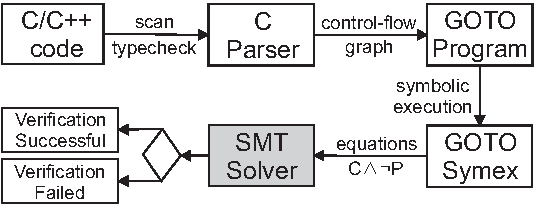
\includegraphics[scale=0.9]{figures/esbmc-arch-new.pdf} 
	\label{ESBMC-Architecture}
\end{figure}

%----------------------------------------------
\subsection{OpenMP}
\label{OpenMP}
%----------------------------------------------

The OpenMP is a set of directives for parallel programming that augments C/C$++$ and Fortran languages, as defined in~\cite{OpenMP1998}. OpenMP supports most processor architectures and operating systems, {\it e.g.}, Solaris, AIX, HP-UX, Linux, Mac OS X, and Windows. OpenMP uses a portable and very robust model to facilitate the development of parallel applications for a variety of platforms. 

In particular, OpenMP uses the \textit{fork-join} model of parallel execution, as shown in~\cite{OpenMP1998}. The main thread executes the sequential parts of the program; if a parallel region is encountered, then it forks a team of worker threads. After the parallel region finishes ({\it i.e.}, the API waits until all threads terminate), then the main procedure returns to the single-threaded execution mode, as shown in~\cite{Wu2014}.

The most basic directive of OpenMP is the ``\textit{\#pragma omp parallel for}'', which parallelizes the enclosing loop; a basic OpenMP example is shown below:

\begin{lstlisting}[basicstyle=\footnotesize,label={lst:example}, language=C, numberstyle=\tiny, numbersep=7pt,frame=tb,captionpos=t, caption={OpenMP basic Example.}]
int k;
#pragma omp parallel for
for (k = 0; k < 10; k++)
  a[k] = 2*k;
\end{lstlisting}

\vspace{2 mm}
In the above example, the {\it for} loop is executed in parallel. Each iteration of the loop is executed in a separated thread; and each thread may use an idle processor. There is also a way to specify critical regions, which is a code block that is guaranteed to be executed by a single thread at a time. To create a critical region, the ``\textit{\#pragma omp critical}'' directive is routinely used.

%----------------------------------------------
\subsection{Solving Optimization Problems with $\nu$Z}
\label{Optimization-with-Vz}
%----------------------------------------------

In this study, the SMT solver Z3 is used to check for the satisfiability of formulas generated from the HW-SW partitioning problem, as shown in~\cite{Bjorner2014}. In particular, we exploit the use of MaxSMT solver $\nu$Z, which is implemented on top of the SMT solver Z3, in order to solve optimization problems; $\nu$Z base function is to optimize objective functions, which formulate optimized criteria, within the logical context of constraints.~$\nu$Z also includes an incremental version of the Maximum Resiliency (MaxRes), as shown in~\cite{Federica2008}, in order to achieve Maximum Satisfiability (MaxSAT), as defined in~\cite{NarodytskaN} and a Simplex to solve numbers without defined patterns. 

In $\nu$Z, MaxSAT is responsible for the restrictions, while OptSMT optimizes linear arithmetic objectives, as shown in~\cite{Bjorner2015}. In summary, $\nu$Z provides three main functions that extend Z3 for solving optimization problems, which are: \textit{maximize}, \textit{minimize}, and \textit{assert-soft}.

\begin{itemize}
\item{\textbf{maximize(T)}
this function instructs the solver that a given variable $T$ should be maximized, which includes real, integer, or bit-vector variables.}
\item{\textbf{minimize(T)}
this function instructs the solver that a given variable $T$ should be minimized, the accepted types are the same as maximize function.}
\item{\textbf{Assert-Soft F : weight n}
the function \textit{assert-soft} adds a restriction to $F$, which can also add a weight $n$; the default value is $1$.}
\end{itemize}

As an example, one can optimize $\left(K + W\right)$, which is subject to restrictions in $\left(K < 2\right)$ and $\left(W - K < 1\right)$. The expected result of this optimization problem described in the code below is $2$. In fact, the model generated by $\nu$Z shows that $K = 1$ and $W = 1$.

\begin{lstlisting}[basicstyle=\footnotesize,language=C,caption={OpenMP basic Example.},label={vZ},numbersep=7pt,frame=tb,captionpos=t,numberstyle=\tiny]
(Declare-Const K Int) 
(Declare-Const W Int)
(assert (< K 2)) 
(assert (< (- W K) 1))
(maximize (+ K W)) 
(check-sat)
\end{lstlisting}

\vspace{2 mm}
Fig.~\ref{vZ-Architecture} shows the $\nu$Z architecture. Initially, the SMT formula with objectives is converted to $0-1$ constraints, which leads to a Pseudo-Boolean Optimization (PBO), as shown in~\cite{Barth1995} and~\cite{Vasco2005}. If there are many objective functions, $\nu$Z invokes OptSAT for arithmetic or MaxSAT for soft constraints. For constraints using real values, $\nu$Z combines linear arithmetic objectives and uses only one instance of OptSMT. When ``soft constrains'' is used in the mode `` lexicographic'', $\nu$Z invokes MaxSAT using multiple calls for its engine.

\begin{figure}[ht]
	\caption{$\nu$Z architecture extracted from~\cite{Bjorner2015}.}
	\centering
	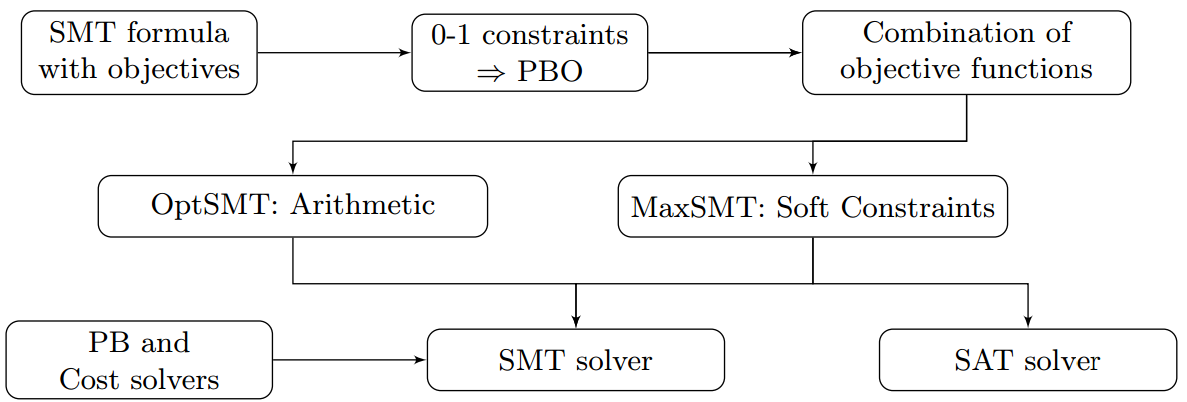
\includegraphics[scale=0.21]{figures/vzArch.png} 
	\label{vZ-Architecture}
\end{figure}

Z3 is available for platforms in C, C$++$, Java, .NET, and Python; it is possible to download Z3 with $\nu$Z from its github repository in~\cite{Z3API}. In this work, the python API is used to formulate HW-SW partitioning problems using the $\nu$Z tool. 

%----------------------------------------------
\section{Mathematical modeling}
\label{Mathematical-modeling}
%----------------------------------------------

The mathematical modeling of the HW-SW partitioning problem was taken from~\cite{Arato2003} and~\cite{Mann2007}.

%----------------------------------------------
\subsection{Informal Model (or Assumptions)}
\label{Informal-Model-or-Assumptions}
%----------------------------------------------

The informal model can be described by five characteristics. First, there is only one software context, {\it i.e.}, there is just one general-purpose processor, and there is only one hardware context. The components of the system must be mapped to either one of these two contexts. Second, the software implementation of a component is associated with a software cost, which is the running time of the component. Third, the hardware implementation of a component has a hardware cost, which can be area, heat dissipation, and energy consumption. Fourth, based on the premise that hardware is significantly faster than software, the running time of the components in hardware is considered as zero. Finally, if two components are mapped to the same context, then there is no overhead of communication between them; otherwise, there is an overhead. The consequence of these assumptions is that scheduling does not need to be addressed in this work. Hardware components do not need scheduling, because the running time is assumed to be zero. Because there is only one processor, software components do not need to be scheduled as well. Therefore, the focus is only on the partitioning problem. That configuration describes a first-generation co-design, where the focus is on bipartitioning, as shown in~\cite{Teich2012}.

%----------------------------------------------
\subsection{Formal Model}
\label{Formal-Model}
%----------------------------------------------

A directed simple graph $ G = (V,E) $, called the task graph of the system, is given. Where the vertices $V = \{V_1,V_2,\dotso,V_n\}$ represent the nodes that are the components of the system that will be partitioned. The edges $E$ represent communication between components. Additionally, each node  $V_i$ has a cost $h(V_i)$ (or $h_i$) of hardware if implemented in hardware and a cost $s(V_i)$ (or $ s_i $) of software if implemented in software. Finally, $c(V_i,V_j)$ represents the communication cost between $V_i$ and $V_j$ if they are implemented in different contexts (hardware or software).

$P$ is called a hardware-software partition if it is a bipartition of $V:P = (V_h, V_s)$, where $V_h \cup V_s = V$  and $V_h \cap V_s = 0$. The crossing edges are $E_p = \{(V_i,V_j):V_i \in V_s, V_j \in V_h$ or $V_i \in V_h, V_j \in V_s $, \cite{Arato2003}. The hardware cost of $P$ is given by Eq.~\ref{hardware-costs}

\vspace{-5 mm}
\begin{align}
\label{hardware-costs}
H_p  &= \Sigma_{V_i \in V_h} h_i,
\end{align}

\vspace{2 mm}
\noindent
and the software cost of $P$ ({\it i.e.}, software cost of the nodes and the communication cost) is given by Eq.~\ref{software-communication-costs}

\vspace{-3 mm}
\begin{align}
\label{software-communication-costs}
  S_p &= \Sigma_{V_i \in V_s}\:s_i + \Sigma_{(V_i,V_j)\in\:E_p} c(V_i,V_j).
\end{align}

\vspace{2 mm}
Different optimization (and decision) problems can be defined, \cite{Arato2003}. In this paper, the focus is on systems with hard real-time constraints: $ S_0 $ is given (initial cost of software), {\it i.e.}, the goal is to find a $P$ HW-SW partitioning so that $ S_p \leq S_0 $ and $ H_p $ is minimal, which is thus related . Based on Eq.~\ref{linear-programming-problem} and~\ref{software-communication-costs}, the constraints can be reformulated as 

\vspace{-2 mm}
\begin{align}
\label{hw-sw-partitioning}
s\left(1-x\right) + c|Ex| \leq S_0, 
\end{align}

\vspace{2 mm}
\noindent where $s$ and $c$ are the vectors representing the cost functions, $E$ is the transposed incidence matrix of $G$ (indicating which edges cross the boundary between the contexts of hardware and software), and $x$ represents the decision variable (a binary vector indicating the partition: 1 if the node is realized in hardware and 0 if node is realized in software). Concerning the complexity of this problem, \cite{Arato2003} demonstrate that it is NP-Hard, as defined in~\cite{Cormem}.

%----------------------------------------------
\section{Analysis of the partitioning problem}
\label{Analysis-of-the-partitioning-problem-using-ESBMC}
%----------------------------------------------

As computer hardware architecture moves from single- to multi-cores, parallel programming environments should be exploited to take advantage of the ability to run several threads on different processing cores. This section describes the verification algorithm using sequential ESBMC, followed by three multi-core model checking algorithms and the integration of the MaxSMT solver $\nu$Z into ESBMC, in order to speed up the HW-SW partitioning verification. HW-SW partitioning using ILP-based and Genetic Algorithms are also explained.

%----------------------------------------------
\subsection{Partitioning problem using ILP-based,Genetic Algorithms}
\label{ILPGA}
%----------------------------------------------

The ILP and GA were taken from our previous studies, from~\cite{Trindade2015} and~\cite{Trindade2016}. Both use slack variables in order to eliminate the modulus operator of Eq.~\ref{hw-sw-partitioning} and to use commercial tools. However, GA had improvements from the parameters of related studies in order to increase the solution accuracy without producing timeout. The tuning was performed by empirical tests and resulted in changing of three parameters, which are passed to the function \textit{ga} of MATLAB, as shown in~\cite{TheMathWorks2013}: the population size was set from $300$ to $500$, the Elite count changed from $2$ (default value) to $50$, and the number of generations changed from $100*NumberOfVariables$ (default) to $75$.

%----------------------------------------------
\subsection{Verification Algorithm using Sequential ESBMC}
\label{Verification-Algorithm-using-ESBMC}
%----------------------------------------------

Figure~\ref{Pseudocode-describing-ESBMC} shows ESBMC pseudocode with the same constraints and conditions placed on ILP and GA. Two values must be controlled to obtain the results and to perform the optimization. One is the initial software cost, as defined in Section~\ref{Formal-Model}. The other is the halting condition (code violation) that stops the algorithm.

The ESBMC algorithm starts with the declarations of hardware, software, and communication costs. $S_0$ must also be defined, as the transposed incidence matrix (used in Eq.~\ref{hw-sw-partitioning}) and the identity matrix (necessary to work with the matrices), as typically done in MATLAB. Here, matrices $A$ and $b$ are generated. At that point, the ESBMC algorithm starts to differ from the ILP and GA presented in~\cite{Trindade2015}.

\begin{lstlisting}[basicstyle=\footnotesize,caption={Pseudocode describing sequential ESBMC.},label={Pseudocode-describing-ESBMC},numbersep=7pt,frame=tb,captionpos=t,numberstyle=\tiny,mathescape=true]
Initialize variables 
Declare number of nodes and edges
Declare hardware cost of each node as array (h)
Declare software cost of each node as array (s)
Declare communication cost of each edge (c)
Declare the initial sw cost of ($S_0$)
Declare transposed incidence matrix graph G(E)
Define the solutions ($x_i$) as Boolean
main {
 For TipH = 0 to Hmax Do {
  Populate $x_i$ with nondet (the values of test)
  Calculate s_i(1-x_i)+c|Ex_i| and store at variable
  Requirement enforced by Assume (variable <= $S_0$)
  Calculate Hp cost Based on value of $x_i$
  Violation check with Assert(Hp > TipH)
 }
}
\end{lstlisting}

\vspace{2 mm}
It is possible to instruct ESBMC with which type of values the variables must be tested. Therefore, there is a declaration to populate all decision variables $x$ with non-deterministic Boolean values. Those values that change for each test will generate a possible solution and obey the constraints. If this is achieved, then a feasible solution is found and the ASSUME directive is responsible for ensuring the compliance of those constrains (\textit{i.e.}, $A.x \leq b$).

A loop controls the cost of hardware hint, starting with zero and reaching the maximum value considering the case, where all nodes are partitioned to hardware (Hmax). To every test performed, the hardware hint is compared to the feasible solution. This is accomplished by an \textit{ASSERT} statement at the end of the algorithm, a predicate that controls the halt condition (a \textit{true-false} statement). If the predicate is \textit{FALSE}, then the optimization is finished, {\it i.e.}, the solution is found. 

The \textit{ASSERT} statement tests the objective function, {\it i.e.}, the hardware cost, and will stop if the hardware cost found is lower than or equal to the optimal solution. However, if \textit{ASSERT} returns a \textit{true} condition, {\it i.e.}, the hardware cost is higher than the optimal solution, then the model-checking algorithm restarts and a new possible solution is generated and tested until the \textit{ASSERT} generates a \textit{false} condition. When the \textit{false} condition happens at verification-time, the execution code is aborted and ESBMC presents the counterexample that caused the condition to be broken. That is the point in which the solution is presented (minimum HW cost).

In the ESBMC algorithm is not necessary to add slack variables at Eq.~\ref{hw-sw-partitioning}, which reduces the number of variables to be solved when compared to ILP and GA. 

%----------------------------------------------
\subsection{Multi-core ESBMC with OpenMP (ESBMC-SS)}
\label{Multi-core-ESBMC-with-OpenMP}
%----------------------------------------------

Typically, ESBMC verification runs are performed only in a single-core. If the processor provides $8$ processing cores, only one is used for the verification and the others remain idle. Thus, there is a significant unused hardware resource during this process. 

To optimize the CPU resources utilization without modifying the underlying SMT solver, the Open Multi-Processing (OpenMP) library, according to~\cite{Dagum1998}, is used in this present work as a front-end for ESBMC. Fig.~\ref{ESBMC-Multi-core} shows our first approach called ESBMC sequential-search ``ESBMC-SS''.

\begin{figure}[h]
	\caption{ESBMC-SS approach.}
	\centering
	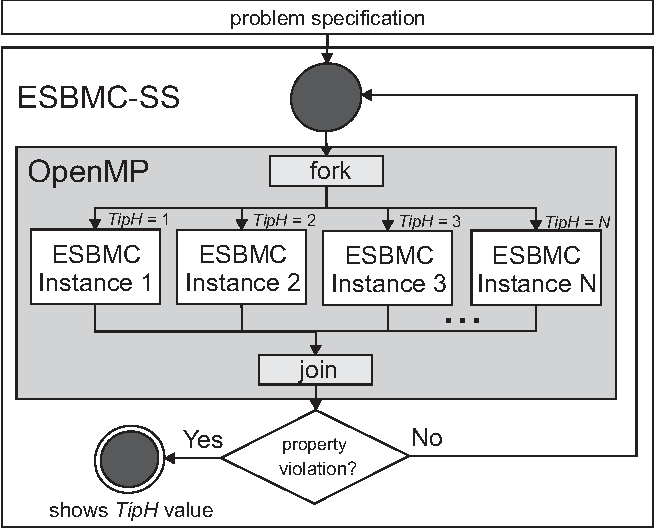
\includegraphics[scale=0.77]{figures/esbmc-ss.pdf} 	
	\label{ESBMC-Multi-core}
\end{figure}

ESBMC-SS obtains the problem specification represented by a ANSI-C program. The HW-SW partitioning is violated, when the correct optimum value (\textit{TipH}) parameter is reached; ESBMC-SS starts a parallel region with different instances of ESBMC, based on the number of available processing cores. All these ESBMC instances run independently of each other, as shown in Fig.~\ref{ESBMC-Multi-core}. Note that there is no shared-memory (or message-passing) mechanism among threads. In particular, different threads are managed by the OpenMP API, which is responsible for the thread life-cycle: start, running, and dead states, using different values as condition. After executing $N$ instances, if there is no code violation, then ESBMC-SS starts new instances again; this represents a sequential-search on a multi-core environment. During the parallel region execution, if a violation is found in any running thread, then it presents a counterexample with the violation condition and the verification time. If all threads of the batch processing are terminated, then ESBMC-SS finishes its execution.

%----------------------------------------------
\subsection{Multi-core ESBMC with OpenMP using Workers (ESBMC-PS)}
\label{Multi-core-ESBMC-with-OpenMP-using-workers}
%----------------------------------------------

The previous parallelization is implemented by continuously forking ESBMC instances in a sequential manner until the first violation is found. However, since OpenMP only returns from a parallelized loop, when every forked thread finishes, some processing cores could remain idle for some period of time.

\begin{figure}[h]
	\caption{ESBMC-PS approach.}
	\centering
	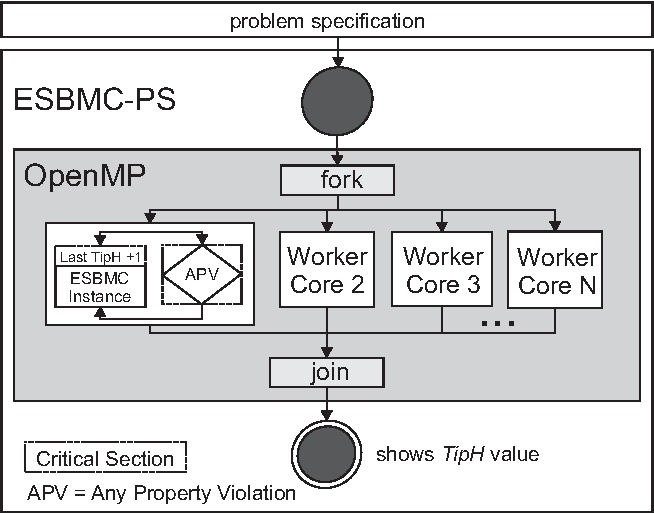
\includegraphics[scale=0.77]{figures/esbmc-ps.pdf} 	
	\label{ESBMC-Multi-core-Optimized-Sequential-Approach}
\end{figure}

\vspace{-5 mm}
Consequently, the second approach aims to remove the idle time from the parallel loops, by creating workers inside threads so that the next step is immediately executed if there is a processing core available, as shown in Fig.~\ref{ESBMC-Multi-core-Optimized-Sequential-Approach}. This approach could potentially lead to great performance improvements, but as ESBMC checks for each step almost at the same rate, the processor does not remain idle for a longer period and thus there is almost no optimization.

%----------------------------------------------
\subsection{Multi-core ESBMC with OpenMP using Binary Search (ESBMC-PB)}
\label{Multi-core-ESBMC-with-OpenMP-using-Binary-Search}
%----------------------------------------------

The most optimized approach applies a parallelized binary-search to reduce the amount of steps to be executed in order to find the optimal solution. A controller is designed to return the step to be executed so that the number of verification runs are substantially reduced. The parallelized binary search accomplishes this by splitting the domain of possible values into intervals and then by returning the middle of the largest interval so that two new intervals are created.

\begin{figure}[ht]
	\caption{ESBMC-PB approach.}
	\centering
	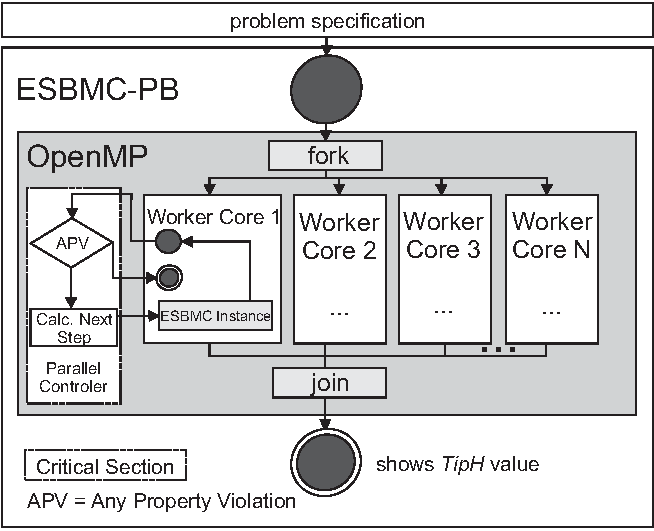
\includegraphics[scale=0.77]{figures/esbmc-pb.pdf} 
	\label{ESBMC-Binary-Approach}
\end{figure}

\vspace{-5 mm}
As an example, given a problem of domain from $1$ to $20$ (see Fig.~\ref{Binary-Step-Calculation}), we firstly create an initial interval from $1$ to $20$. When the next available core requests a step to be executed, the controller obtains the largest interval, {\it i.e.}, $\left[1,20\right]$, divides it by two, which creates two new intervals ({\it i.e.}, $\left[1,9\right]$ and $\left[11,20\right]$), and returns the middle of the original interval ({\it i.e.}, $10$). The controller also checks whether an interval has less than two elements to avoid creating empty or invalid intervals.

\begin{figure}[h!]
	\caption{Binary step calculation.}
	\centering
	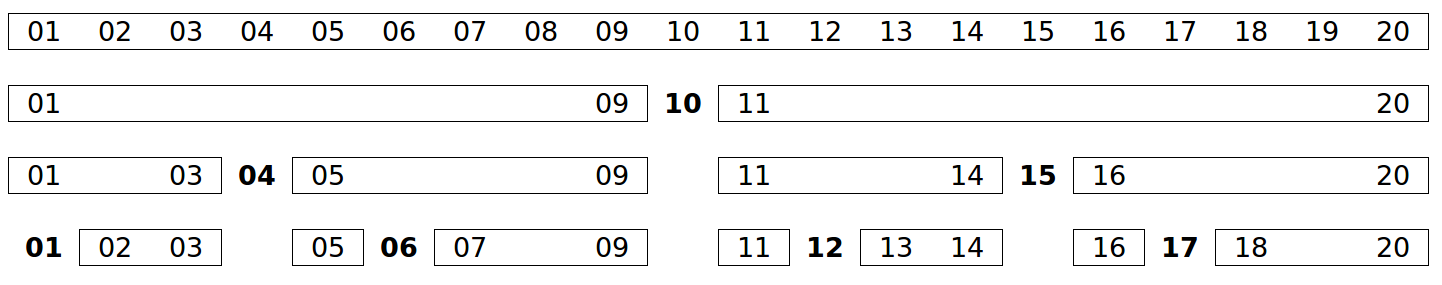
\includegraphics[scale=0.17]{figures/Fig4.png}	
	\label{Binary-Step-Calculation}
\end{figure}

\vspace{-4 mm}
Note that there might gaps between steps, which are produced by the customized binary-search. For instance, in the example shown in Fig.~\ref{Binary-Step-Calculation}, if step $10$ returns \textit{false}, then one can conclude that all steps after $10$ is \textit{false} as well. However, if the same step $10$ returns \textit{true}, we can assume that all steps before $10$ is \textit{true} as well. As a result, an auxiliary method to remove unnecessary steps is implemented in the controller by removing or shrinking existing intervals. This approach leads to a high impact in the verification time. However, if a step is running and is not needed anymore, the worker kills the forked process and starts a new one.

Algorithm in Figure~\ref{Steps-Calculation-using-Intervals} describes how the customized binary search calculates and returns the step to be executed. 

Note that algorithm of Figure~\ref{Steps-Calculation-using-Intervals} is called from each worker in order to get the next step to execute if it exists; otherwise, either zero or a negative number is returned.
From lines $4$ to $9$, the algorithm finds the largest interval. Then, from line $10$ the largest interval is removed and the median is calculated in line $11$. After that, two new intervals are created, the left side (in line $14$) and the right side (in line $18$). At the end, the median is returned.

\vspace{-1.5 mm}
\begin{lstlisting}[basicstyle=\footnotesize,caption={Steps calculation using intervals.},label={Steps-Calculation-using-Intervals},numbersep=7pt,frame=tb,captionpos=t,numberstyle=\tiny]
GetNextStep(){
 int largestChunk = -1;
 chunk largest;
 for each(chunk in chunks){
  if(chunk.right - chunk.left > largestChunk){
    largestChunk = chunk.right - chunk.left;
    largest = chunk;
  }
 }	
 chunks.remove(largest);	
 int median = largest.left + 
   floor((largest.right - largest.left) / 2);
 if(median > 0){
  if(largest.right - largest.left > 1)
   chunks.add(
     new chunk(largest.left, median - 1)
   );	
  if(largest.right != largest.left)
   chunks.add(
    new chunk(median + 1, largest.right)
   );
 }
 return median;
}
\end{lstlisting}

\vspace {-1.5 mm}
Algorithm of Figure~\ref{worker-sample} describes how the worker starts and monitors ESBMC instances. The algorithm starts by retrieving the step to be executed from the controller (line $1$), then initiates the ESBMC instance and obtains the process \textit{id} from the forked process (line $2$). While the step is being executed, the controller checks whether this step is still needed (line $4$). If not, then the ESBMC instance is killed (line $5$) and the worker is free to initiate another step.

\begin{lstlisting}[basicstyle=\footnotesize,caption={Worker sample.},label={worker-sample},numbersep=7pt,frame=tb,captionpos=t,numberstyle=\tiny]
step = controller.GetNextStep();
int pid = ExecuteStep(step);
while(isRunning(pid)){
 if(!controller.isNeeded(step))
   kill(pid);
}
\end{lstlisting}

%----------------------------------------------
\subsection{Analysis of the partitioning problem using $\nu$Z (ESBMC-$\nu$Z)}
\label{Analysis-of-the-partitioning-problem-using-vZ}
%----------------------------------------------

Algorithm of Figure~\ref{vZ-pseudocode} encodes the objective function and constraints related to the HW-SW partitioning problem using $\nu$Z functions, as seen in~\cite{Bjorner2014}. A $\nu$Z logical context must firstly be created (line $2$), in order to add constraints and to check whether a given model exists to the set of constraints. Note that the number of nodes and edges, software, hardware, and communications costs as well as the incidence matrix E must also be declared.

The arithmetic expressions from lines $10$ to $12$ represent the constraints described in Eq.~\ref{hw-sw-partitioning}. Here, variable \textit{SC} refers to the software cost, while \textit{CC} denotes the communication cost. In line $12$, the \textit{Fobj} (objective function) is declared, which denotes the product between the hardware cost and the decision variables vector, which contains only Boolean values. \textit{Fobj} should be minimized to obtain the optimal hardware solution. To achieve this, two constraints are imposed to ESBMC-$\nu$Z: the first one refers to the sum of the software and communication costs, where the result should be less than $S_0$; and the second one instructs to ESBMC-$\nu$Z that \textit{Fobj} should be minimized. Finally, the model is checked by ESBMC-$\nu$Z and if there is a solution that 
meets the constraints, then the \textit{Fobj} value is provided.

\begin{lstlisting}[basicstyle=\footnotesize,caption={Pseudocode describing ESBMC-$\nu$Z.},label={vZ-pseudocode},numbersep=7pt,frame=tb,captionpos=t,numberstyle=\tiny,mathescape=true]
-Initialize Variables
 Create vZ context 
 Create binary vector (x)
 Declare number of nodes, edges and $S_0$
 Declare hardware cost of each node as array (h) 
 Declare software cost of each node as array (s)
 Declare communication cost of each edge (c)
 Declare transposed incidence matrix graph G(E)
-Arithmetic Expressions
 SC = s(1-x)
 CMC = c*|EX|
 Fobj =  x[i] * h[i]
-Assert Constraints
 Add constraints (SF + CMC <= $S_0$)
 Add constraints to minimize Fobj
 Check Model
 Print Result
\end{lstlisting}

\vspace {-2 mm}
%----------------------------------------------
\section{Experimental Evaluation}
\label{Experimental-Evaluation}
%----------------------------------------------

This section is split into three parts. The setup is described in Section~\ref{Experimental-Setup}, while Section~\ref{Benchmarks-Description} describes all benchmarks that were used for performing the experimental evaluation. Section~\ref{Experimental-Results} reports a comparison among MATLAB, ESBMC-SS, ESBMC-PS, ESBMC-PB, and ESBMC-$\nu$Z using a set of standard HW-SW partitioning benchmarks, as shown in~\cite{Mann2007}.

%----------------------------------------------
\subsection{Experimental Setup}
\label{Experimental-Setup}
%----------------------------------------------

ESBMC v$2$.$0$ running on a $64$-bit Ubuntu $14$.$04$.$1$ LTS operating system was used. A parallel approach of the ESBMC-SS, ESBMC-PS, ESBMC-PB were implemented in C$++$11. Version $2$.$0$.$1$ of Boolector SMT-solver, as shown in~\cite{Brummayer2009} (freely available) was used as the default solver for ESBMC. ESBMC-$\nu$Z as a built-in tool to Z3 was also used, as shown in~\cite{Bjorner2014}.  For ILP and GA formulations, MATLAB R$2013$a from MathWorks with Parallel Computing Toolbox was used, as shown in~\cite{TheMathWorks2013}. MATLAB is a dynamically typed high-level language, known as the state-of-the-art mathematical software, as shown in~\cite{Tranquillo2011} and is widely used by the engineering community, as shown in~\cite{Hong2010}.

All experiments were conducted on an otherwise idle Intel Core i$7$-$2600$ ($8$-cores), with $3$.$4$ GHz and $24$ GB of RAM, running Ubuntu $64$-bits. Each time was measured $3$ times (average taken). Based on standard deviation and tolerance interval to each set of time sample, it was obtained a statistical confidence of $91.7$\% to ESBMC (sequential, SS, PB and $\nu$Z), $95.9$\% to ESBMC-PS, and $92.0$\% to ILP and GA. A timeout condition (TO) is reached when the verification time is longer than $3600$ seconds. A memory-out (MO) occurs when the tool reaches $15$ GB of memory. 

%----------------------------------------------
\subsection{Description of Benchmarks}
\label{Benchmarks-Description}
%----------------------------------------------


\begin{minipage}{\linewidth}
\centering
\small
\sffamily\small
\tabulinesep=4pt
\captionof{table}{Description of Benchmarks.} 
\begin{tabular}[c]{m{1.5cm}m{0.7cm}m{0.7cm}m{4.0 cm}}
\toprule[1.5pt]
\textbf{Name} & \textbf{Nodes} & \textbf{Edges} & \textbf{Description}\\
\midrule
\verb|CRC32| & \verb|25| & \verb|32| & \rmfamily 32-bit cyclic redundancy check, as shown in~\cite{Guthaus2001}\\
\hline
\verb|Patricia| & \verb|21| & \verb|48| & \rmfamily
\vspace{0.8 mm} Routine to insert values in Patricia Tree, as shown in ~\cite{Guthaus2001}\\
\hline
\verb|Dijkstra| & \verb|26| & \verb|69| & \rmfamily \vspace{0.8 mm} Computer shortest paths in a graph, as shown in~\cite{Guthaus2001}\\
\hline
\verb|Clustering| & \verb|150| & \verb|331| & \rmfamily \vspace{0.8 mm} Image segmentation algorithm in a medical application\\
\hline
\verb|RC6| & \verb|329| & \verb|448| & \rmfamily \vspace{0.8 mm} RC6 cryptography graph algorithm\\
\hline
\verb|Fuzzy| & \verb|261| & \verb|422| & \rmfamily \vspace{0.8 mm} Clustering algorithm based on fuzzy logic\\
\hline
\verb|Mars| & \verb|417| & \verb|600| & \rmfamily 
\vspace{1 mm} MARS cipher from IBM algorithm\\
\bottomrule[1.5pt]
\label{tab:Description-of-Benchmarks} 
\end{tabular}\par
\bigskip
\end{minipage}

\vspace{-3 mm}
To perform the experiments, some benchmarks provided by~\cite{Mann2007} were used, as shown in Table~\ref{tab:Description-of-Benchmarks}. The nodes in the graphs correspond to high-level language instructions. Software and communication costs are time dimensional, and hardware costs represent the occupied area. The first three benchmarks are extracted from MiBench, as shown in~\cite{Guthaus2001}. The clustering and fuzzy benchmarks are designed from~\cite{Mann2007} and are significantly large benchmarks. From the same authors, very complex benchmarks to test the limits of the applicability of techniques were used (RC$6$ and Mars).

%----------------------------------------------
\subsection{Experimental Results}
\label{Experimental-Results}
%----------------------------------------------

Table~\ref{Experimental-results-of-the-complex-benchmarks} shows the experimental results using Matlab (ILP and GA) and ESBMC (ESBMC-SS, ESBMC-PS, ESBMC-PB, ESBMC-$\nu$Z) tools.

There is no single tool for efficiently solving all HW-SW partitioning benchmarks. In particular, the best (proposed) solution is ESBMC-$\nu$Z, which solves $4$ out of $7$ benchmarks; ESBMC-$\nu$Z is faster than ILP in all supported benchmarks ({\it i.e.}, CRC$32$, Patricia, Dijkstra, Clustering), but it returns three TOs (timeouts) related to RC6, Fuzzy and Mars benchmarks.

In contrast to ESBMC-$\nu$Z, ILP solves $5$ out of $7$ benchmarks. When ILP produces a result, it provides the optimal solution. On the one hand, ILP execution time is slower than $\nu$Z in all benchmarks, which are supported by ESBMC-$\nu$Z. On the other hand, ILP is faster than ESBMC-SS, ESBMC-PS, and ESBMC-PB in all benchmarks, except for the clustering.

Note further that all multi-core ESBMC implementations produce better results than the sequential one. In particular, ESBMC-PB implementation outperforms all other multi-core ESBMC approaches, where its performance improves as the number of nodes and edges increase. One notable case is the clustering benchmark, when verified by ESBMC-PB, it executes $3$ times faster than ILP and $2$.$5$ times slower than ESBMC-$\nu$Z. However, when the amount of nodes is around $30$, ESBMC-PB does not outperform ESBMC-$\nu$Z and ILP tools. When analyzing all benchmarks, ESBMC-PB produces TO for RC$6$, Fuzzy, and Mars; however, the results are still promising if we take into consideration that $\nu$Z and Matlab are state-of-the-art tools with respect to optimization problems.

\begin{table*}[ht]
  \centering
  \caption{Experimental results of the HW-SW partitioning benchmarks.}  
  \begin{tabular}{*{9}{cc|c|c|c|c|c|c|c}}
\\
 &  & \rotatebox{90}{\textbf{\normalsize{CRC32}}} & \rotatebox{90}{\textbf{\normalsize{Patricia}}} & \rotatebox{90}{\textbf{\normalsize{Dijkstra}}} & \rotatebox{90}{\textbf{\normalsize{Clustering}}} & \rotatebox{90}{\textbf{\normalsize{RC6}}} & \rotatebox{90}{\textbf{\normalsize{Fuzzy}}} & \rotatebox{90}{\textbf{\normalsize{Mars}}} \\[0.15cm]
\cmidrule(r){3-9}

&\textbf{\normalsize{Nodes}} &\normalsize{25} & \normalsize{21} & \normalsize{26} & \normalsize{150} & \normalsize{329} & \normalsize{261} & \normalsize{417}\\
&\textbf{\normalsize{Edges}} &\normalsize{32} & \normalsize{48} & \normalsize{69} & \normalsize{331} & \normalsize{448} & \normalsize{442} & \normalsize{600}\\
&\textbf{\normalsize{S0}} &\normalsize{20} & \normalsize{10} & \normalsize{20} & \normalsize{50} & \normalsize{600} & \normalsize{4578} & \normalsize{300} \\

\bottomrule[1.5pt]
\rowcolors{1}{}{lightgray}

\multirow{4}{*}{\textbf{\normalsize{Exact Solution}}}
& & & & & & & & & \\
&  \normalsize{Hp}   &  \normalsize{15}   &  \normalsize{47}   &  \normalsize{31}   &  \normalsize{241} &  \normalsize{692} &  \normalsize{13820}   &  \normalsize{876} \\
&  \normalsize{Sp}   &  \normalsize{19}   &  \normalsize{4}   &  \normalsize{19}   &  \normalsize{46}   &  \normalsize{533}    &  \normalsize{4231}   &  \normalsize{297}  \\
& & & & & & & & & \\

\bottomrule[1.5pt]
%ILP
\multirow{4}{*}{\textbf{\normalsize{ILP}}}
& & & & & & & & & \\
&  \normalsize{T(s)}   &  \normalsize{1.6}   &  \normalsize{1.3}  &  \normalsize{1.6}   &  \normalsize{648.9}   &  \normalsize{1806.2}    &  \normalsize{TO}   &  \normalsize{TO}  \\
&  \normalsize{Hp}   &  \normalsize{15}  &  \normalsize{47}   &  \normalsize{31}   &  \normalsize{241}   &  \normalsize{692}    &  -   &  -  \\
& & & & & & & & & \\
\hline

%GA
\multirow{4}{*}{\textbf{\normalsize{{GA}}}}
& & & & & & & & & \\
&  \normalsize{T(s)}   &  \normalsize{6.7}   &  \normalsize{7.4}   &  \normalsize{8.8}   &  \normalsize{340.4}   &  \normalsize{2050.0}    &  \normalsize{1371.9}   &  \normalsize{TO}  \\
&  \normalsize{Error \%}   &  \normalsize{13.3}   &  \normalsize{0.0}   &  \normalsize{29.0}   &  \normalsize{1.7}   &  \normalsize{-6.5}    &  \normalsize{-37.6}   &  -  \\
& & & & & & & & & \\
\hline

%ESBMC
\multirow{4}{*}{\textbf{\normalsize{{ESBMC}}}}
& & & & & & & & & \\
&  \normalsize{T(s)}   & \normalsize{30.3}   &  \normalsize{313.7}   &  \normalsize{324.7}   &  \normalsize{MO}   & \normalsize{MO}    &  \normalsize{MO}   &  \normalsize{MO } \\
&  \normalsize{Hp}   &  \normalsize{15}   &  \normalsize{47}   &  \normalsize{31}   &  -   &  -    &  -   &  -  \\
& & & & & & & & & \\
\hline

%MultiCore ESBMC
\multirow{4}{*}{\textbf{\normalsize{{ESBMC-SS}}}}
& & & & & & & & & \\
&  \normalsize{T(s)}   & \normalsize{2.2}  &  \normalsize{5.8}   &  \normalsize{7.0}  &  \normalsize{1609.3}   &  \normalsize{TO}    &  \normalsize{TO}   &  \normalsize{TO}  \\
&  \normalsize{Hp}   &  \normalsize{15}   &  \normalsize{47}   &  \normalsize{31 }  &  \normalsize{241 }  &  -    &  -   &  -  \\
& & & & & & & & & \\
\hline

%ESBMC Parallel sequential
\multirow{4}{*}{\textbf{\normalsize{ESBMC-PS}}}
& & & & & & & & & \\
&  \normalsize{T(s)} &  \normalsize{3.7} &  \normalsize{10.0}   &  \normalsize{12.0}   &  \normalsize{2468.0}   &  \normalsize{TO}    &  \normalsize{TO}   &  \normalsize{TO}  \\
&  \normalsize{Hp}   &  \normalsize{15}   &  \normalsize{47}   &  \normalsize{31}   &  \normalsize{241}   &  -    &  -   &  -  \\
& & & & & & & & & \\
\hline

%ESBMC Parallel Binary
\multirow{4}{*}{\textbf{\normalsize{{ESBMC-PB}}}}
& & & & & & & & & \\
&  \normalsize{T(s)}   &  \normalsize{4.3}   & \normalsize{4.7}   &  \normalsize{6.3}   &  \normalsize{218.7}   &  \normalsize{TO}    & \normalsize{TO}   & \normalsize{TO} \\
&  \normalsize{Hp}   &  \normalsize{15}   &  \normalsize{47}   &  \normalsize{38}   &  \normalsize{241}   &  -    &  -   &  -  \\
& & & & & & & & & \\
\hline

%vZ
\multirow{4}{*}{\textbf{\normalsize{{ESBMC-$\nu$Z}}}}
& & & & & & & & & \\
&  \normalsize{T(s)}   &  \normalsize{0.3}   & \normalsize{0.3}   &  \normalsize{0.7}   &  \normalsize{86.4}   &  \normalsize{TO}    &  \normalsize{TO}   &  \normalsize{TO } \\
&  \normalsize{Hp}   &  \normalsize{15}   &  \normalsize{47}   &  \normalsize{31}   &  \normalsize{241}   &  -    &  -   &  -  \\
& & & & & & & & & \\

\bottomrule[1.5pt]
\end{tabular}
\label{Experimental-results-of-the-complex-benchmarks}
\end{table*}

The only technique that is able to solve all benchmarks is GA; however, its precision is not satisfactory since it produces an error rate between $-37.6$\% and $29.0$\%.

Note that RC$6$ produced timeouts for all implementations of ESBMC; GA did not produce the correct answer, and ILP solves correctly most benchmarks, except for Mars and Fuzzy, which produced timeouts and memory-outs in all tools that aim to find the exact solution. No tool was capable to solve Mars in less than $3600$ seconds, while GA solved all benchmarks, but mostly incorrectly.

The clustering benchmark seems to be the limit to test the ESBMC (described) implementations; note, however, that more than $150$ nodes lead to TO and MO. ILP shows robustness and produces results even for a high number of nodes and edges, but limited to $329$ nodes.

%----------------------------------------------
\section{Related Work}
\label{Related-Work}
%----------------------------------------------

Since the second half of the first decade of 2000s, three main paths have been tracked to improve or to present alternative solutions to the optimization of HW-SW partitioning, {\it i.e.}, to find the exact solution, as shown in~\cite{Mann2007}; to use heuristics to speed up performance time, as shown in~\cite{Arato2003}; and hybrid ones, as shown in~\cite{Arato2005}.

In the first group, the exact solution to the HW-SW partitioning problem is found. The use of SMT-based verification presented in this paper can be grouped into this category, because the exact solution is found with the given algorithms. The difference is based only on the technique chosen to solve the problem.
Another path followed in past initiatives and which has had more studies is the creation of heuristics to speed up the running time of the solution. The difference of this kind of solution to SMT-based verification and maximum satisfiability is based on two facts: all ESBMC implementations guarantee to find the exact solution, but heuristics are faster, when the complexity is greater.

Finally, there are approaches that mixes heuristics with exact solution tools. The idea is to use a heuristic to speed up some phase of an exact solution tool. It worth mentioning that the final solution is not necessarily an optimal global solution. Only the SMT-based verification is guaranteed to find the exact solution, but hybrid algorithms are faster when complexity rises.

In terms of SMT-based verification, most related studies are restricted to present the model, its modification to programming languages ({\it e.g.}, C/C++ and Java), and the application to multi-thread algorithms or to embedded systems to check for program correctness. In~\cite{Ramalho2013} it presents a bounded model checker for C++ programs, which is an evolution of dealing with C programs, and~\cite{Cordeiro2012} uses ESBMC for embedded ANSI-C software. In~\cite{Trindade2015}, and~\cite{Trindade2016} it was proven that it is possible to use ESBMC to solve HW-SW partitioning in a single- and multi-core way, but the former has performance issues that were improved by the latter, which used only a sequential search to perform multi-core model checking. There are related studies focused on decreasing the verification time of model checkers by applying Swarm Verification, as shown in~\cite{Holzmann2011}, and modifications of internal search engines to add support for parallelism, as shown in~\cite{Holzmann2012}, but there is still the need for initiatives related to parallel SMT solver, according to~\cite{Wintersteiger2009}. 

Recently, the SMT solver Z3 has been extended to pose and solve optimization problems modulo theories, as shown in~\cite{Bjorner2015}. In particular, $\nu$Z tool offers substantial performance improvement in optimization problems, according to~\cite{Bjorner2014} and~\cite{Bjorner2015}. As an application example, \cite{Pavlinovic2015} propose an approach which considers all possible compiler error sources for statically typed functional programming languages and reports the most useful one subject to some usefulness criterion. The authors formulate this approach as an optimization problem related to SMT and use $\nu$Z to compute an optimal error source in a given ill-typed program. The approach described by \cite{Pavlinovic2015}, which uses MaxSMT solver $\nu$Z, shows a significant performance improvement if compared to previous SMT encodings and localization algorithms.

The problem addressed in this present paper uses a single objective function for minimization. In~\cite{Patrick2015}, OptiMathSAT and $\nu$Z are compared for software optimization problems. OptiMathSAT, using multiple objective functions, works better than $\nu$Z; however, for problems with a single objective function, the performance of $\nu$Z is better than OptiMathSAT.

\vspace {-4 mm}
%----------------------------------------------
\section{Conclusions}
\label{Conclusions}
%----------------------------------------------

We presented five approaches to solve the HW-SW partitioning problem and compared them to other state-of-the-art techniques. Experimental results showed that for a number of nodes larger than $300$, the best solution for the HW-SW partitioning problem is ILP. Below that, the best solution turns out to be ESBMC-$\nu$Z since its execution time is faster and notorious. ESBMC-PB is a viable alternative for a number of nodes lower than $150$. GA had an intermediate result in terms of performance, but the error presented from exact solution made it not acceptable to that kind of application. 

If considering off-the-shelf tools, as MATLAB to ILP and GA, the coding is simpler. However, ESBMC and $\nu$Z have BSD-Style and MIT licenses, respectively and can be downloaded and used for free. Experimental results also pointed to an improvement of ESBMC, when using a parallel approach. In particular, all three parallel approaches described in this paper produced expressive results. The fastest ESBMC approaches is ESBMC-PB, which produces good results for an intermediate amount of edges and nodes. Thus, considering that nowadays processors have more and more cores, when modeling the problem, it is possible to consider multi-core model checking as an alternative to solve the HW-SW partitioning problem. 

Finally, there is an issue about $150$ nodes problem, since it seems to be the limit of multi-core ESBMC. However, it really depends on the modeling granularity of the problem. Some researchers propose fine-grained models, in which each instruction can be mapped to either HW or SW. This may lead to thousands of nodes or even more. Others defend coarse-grained models, where decisions are made for larger components, thus even complex systems may consist of just some dozens of nodes to partition. In principle, a fine-grained approach may allow to obtain better partitions, but at the cost of an exponential increase of the search space size. In future work, we will address improvements in ESBMC to remove the parallel layer on top of ESBMC and implement it during symbolic execution so that we can optimize the overall verification time.

\begin{thebibliography}{10}

\bibitem[\protect\citeauthoryear{Arato \textit{et al.}}{2003}]{Arato2003}
Arato, P., Juhasz, S., Mann, A., Orban, A. and Papp, D. (2003) 'Hardware/software partitioning in embedded system design', {\it International Symposium on Intelligent Signal Processing}, pp.192--202

\bibitem[\protect\citeauthoryear{Mann \textit{et al.}}{2007}]{Mann2007}
Mann, A., Orban, A. and Arato, P. (2007) 'Finding optimal hardware/software partitions', {\it Formal Methods in System Design}, Vol. 31, No. 3, pp.241--263

\bibitem[\protect\citeauthoryear{Trindade and Cordeiro}{2015}]{Trindade2015}
Trindade, A. and Cordeiro, L. (2015) 'Applying SMT-based verification to hardware/software partitioning in embedded systems', {\it Design Automation for Embedded Systems (to appear)}

\bibitem[\protect\citeauthoryear{Trindade \textit{et al.}}{2015}]{Trindade2016}
Trindade, A., Ismail, H. and Cordeiro, L. (2015) 'Applying Multi-Core Model Checking to Hardware-Software Partitioning in Embedded Systems (short paper)', {\it V Brazilian Symposium on Computing Systems Engineering (to appear)}

\bibitem[\protect\citeauthoryear{Bjorner \textit{et al.}}{2015}]{Bjorner2015}
Bjorner, N., Phan, A. and Fleckenstein, L. (2015) 'vZ - An Optimizing SMT Solver', {\it Proceedings of the International Conference on Tools and Algorithms for the Construction and Analysis of Systems}, Vol. 9035, pp.194--199

\bibitem[\protect\citeauthoryear{Tang \textit{et al.}}{2010}]{Tang2009}
Tang, T., Lin, Y. and Ren, X. (2010) 'Mapping OpenMP concepts to the stream programming model', {\it Proceedings of the International Conference on Computer Science Education}, pp.1900--1905

\bibitem[\protect\citeauthoryear{Muller}{2002}]{OpenMP1998}
Muller, M. (2002) 'OpenMP Architecture Review Board, OpenMP C and C++ Application Program Interface, Version 2.0', {\it OpenMP Architecture Review Board}

\bibitem[\protect\citeauthoryear{Cordeiro \textit{et al.}}{2012}]{Cordeiro2012}
Cordeiro, L. Fischer, B. and Marques-Silva, J. (2012) 'SMT-based Bounded Model Checking for Embedded ANSI-C Software', {\it IEEE Transactions on Software Engineering}, Vol. 38, No. 4, pp.957--974

\bibitem[\protect\citeauthoryear{Rao}{2009}]{Rao2009}
Rao, S. (2009) 'Engineering Optimization: Theory and Practice. 4th edition'

\bibitem[\protect\citeauthoryear{Biere \textit{et al.}}{2009}]{Biere2009}
Biere, A., Heule, M., Maaren, H. and Walsh, T. {2009} 'Bounded Model Checking', {\it Handbook of Satisfiability}

\bibitem[\protect\citeauthoryear{Clarke \textit{et al.}}{2001}]{Clarke2001}
Clarke, E., Biere, A., Raimi, R. and Zhu, Y. (2001) 'Bounded model checking using satisfiability solving', {\it Formal Methods in System Design}, Vol. 19, No. 1, pp.7--34

\bibitem[\protect\citeauthoryear{Armando \textit{et al.}}{2009}]{Armando2009}
Armando, A., Mantovani, J. and Platania, L. (2009) 'Bounded model checking of software using SMT solvers instead of SAT solvers', {\it International Journal on Software Tools for Technology Transfer}, Vol. 11, No. 1, pp.69--83

\bibitem[\protect\citeauthoryear{Ganai and Gupta}{2006}]{Ganai2006}
Ganai, M. K. and Gupta, A. (2006) 'Accelerating high-level bounded model checking', {\it Proceedings of the IEEE/ACM International Conference on Computer-Aided Design}, pp.794--801

\bibitem[\protect\citeauthoryear{Ramalho \textit{et al.}}{2013}]{Ramalho2013}
Ramalho, M., Freitas, M., Sousa, F., Marques, H., Cordeiro, L. and Fischer, B. (2013) 'SMT-Based Bounded Model Checking of C++ Programs', {\it International Conference and Workshops on the Engineering of Computer-Based Systems}, pp.147--156

\bibitem[\protect\citeauthoryear{Moura and Bjorner}{2008}]{DeMoura2008}
Moura, L. and Bjorner, N. (2008) 'Z3: An Efficient SMT Solver', {\it Proceedings of the International Conference on Tools and Algorithms for the Construction and Analysis of Systems}, pp.337--340

\bibitem[\protect\citeauthoryear{Brummayer and Biere}{2009}]{Brummayer2009}
Brummayer, R. and Biere, A. (2009) 'Boolector: An Efficient SMT Solver for Bit-Vectors and Arrays', {\it Proceedings of the International Conference on Tools and Algorithms for the Construction and Analysis of Systems}, Vol. 5505, pp.174--177

\bibitem[\protect\citeauthoryear{Barrett \textit{et al.}}{2011}]{Barrett2011}
Barrett, C., Conway, C., Deters, M., Hadarean, L., Jovanovic, D., King, T., Reynolds, A. and Tinelli, C. (2011) 'CVC4', {\it Proceedings of the International Conference on Computer-Aided Verification}, Vol. 6806, pp.171--177

\bibitem[\protect\citeauthoryear{Bozzano \textit{et al.}}{2005}]{Bozzano2005}
Bozzano, M., Bruttomesso, R., Cimatti, A., Junttila, T., Rossum, P., Schulz, S. and Sebastiani, R. (2005) 'MathSAT: Tight integration of SAT and mathematical decision procedures', {\it Journal of Automated Reasoning}, Vol. 35, No. 1-3, pp.265--293

\bibitem[\protect\citeauthoryear{Dutertre}{2014}]{Dutertre2014}
Dutertre, B. (2014) 'Yices 2.2', {\it Proceedings of the International Conference on Computer-Aided Verification}, Vol. 8559, pp.737--744

\bibitem[\protect\citeauthoryear{Wu \textit{et al.}}{2014}]{Wu2014}
Wu M., Wu, W., Tai, N., Zhao, H., Fan, J. and Yuan, N. (2014) 'Research on OpenMP model of the parallel programming technology for homogeneous multicore DSP', {\it Proceedings of the International Conference on Software Engineering and Service Science}, pp.921--924

\bibitem[\protect\citeauthoryear{Bjorner and Phan}{2014}]{Bjorner2014}
Bjorner, N. and Phan, A (2014) 'vZ - Maximal Satisfaction with Z3', {\it Proceedings of the International Symposium on Symbolic Computation in Software Science}, pp.1--10


\bibitem[\protect\citeauthoryear{Paci \textit{et al.}}{2008}]{Federica2008}
Paci, F., Ferrini, R., Sun, Y. and Bertino, E. (2008) 'Authorization and User Failure Resiliency for WS-BPEL business processes', {\it Proceedings of the International Conference on Service-Oriented Computing}, pp.116--131

\bibitem[\protect\citeauthoryear{Narodytska and Bacchus}{2014}]{NarodytskaN}
Narodytska, N. and Bacchus, F. (2014) 'Maximum Satisfiability Using Core-Guided MAXSAT Resolution', {\it Proceedings of the Conference on Artificial Intelligence}, pp.2717--2723

\bibitem[\protect\citeauthoryear{Barth and Putnam}{1995}]{Barth1995}
Barth, P. and Putnam, D. (1995) 'Enumeration Algorithm for Linear Pseudo-Boolean Optimization', {\it Technical Report MPI-I-95-2-003, Max Plank Institute for Computer Science}

\bibitem[\protect\citeauthoryear{Manquinho and Marques-Silva}{1995}]{Vasco2005}
Manquinho, V. and Marques-Silva, J. (1995) 'Effective Lower Bounding Techniques for Pseudo-Boolean Optimization', {\it IST/INESC-ID, Technical University of Lisbon, Portugal}

\bibitem[\protect\citeauthoryear{Microsoft Research}{2015}]{Z3API}
Microsoft Research (2015) 'Z3 API - Source code and documentation' [online] {\it https://z3.codeplex.com/} (Accessed 18 August 2015)

\bibitem[\protect\citeauthoryear{Cormen \textit{et al.}}{2009}]{Cormem}
Cormen, T., Leiserson, C., Rivest, R. and Stein, C. (2009) 'Introduction to Algorithms', {\it MIT Press}, Vol. I-XIX, pp.1--1292

\bibitem[\protect\citeauthoryear{Dagum and Menon}{1998}]{Dagum1998}
Dagum, L. and Menon, R. (1998) 'OpenMP: An Industry-Standard API for Shared-Memory Programming', {\it Proceedings of the International Conference on Computational Science Engineering}, pp.46--55

\bibitem[\protect\citeauthoryear{MathWorks}{2013}]{TheMathWorks2013}
MathWorks Inc. (2013) 'MATLAB (version R2013a)'

\bibitem[\protect\citeauthoryear{Tranquillo}{2011}]{Tranquillo2011}
Tranquillo, J. (2011) 'Matlab for Engineering and the Life Sciences', {\it Synthesis Lectures on Engineering. Morgan Claypool}

\bibitem[\protect\citeauthoryear{Hong and Cai}{2010}]{Hong2010}
Hong, L. and Cai, J. (2010) 'The application guide of mixed programming between MATLAB and other programming languages', {\it Proceedings of the International Conference on Computer and Automation Engineering}, pp.185--189

\bibitem[\protect\citeauthoryear{Cordeiro and Fischer}{2011}]{Cordeiro2011}
Cordeiro, L. and Fischer, B. (2011) 'Verifying multi-threaded software using SMT-based context-bounded model checking', {\it Proceedings of the International Conference on Software Engineering}, pp.331--340

\bibitem[\protect\citeauthoryear{Teich}{2012}]{Teich2012}
Teich, J. (2012) 'Hardware/Software Codesign: The Past, the Present, and Predicting the Future', {\it Proceedings of the IEEE, Special Centennial Issue}, Vol. 100, pp.1411--1430

\bibitem[\protect\citeauthoryear{Guthaus \textit{et al.}}{2011}]{Guthaus2001}
Guthaus, M., Ringenberg, J., Ernst, D., Austin, T., Mudge, T. and Brown, R. (2011) 'MiBench: A free, commercially representative embedded benchmark suite', {\it Proceedings of the annual workshop on workload characterization}, pp.3--14

\bibitem[\protect\citeauthoryear{Arato \textit{et al.}}{2005}]{Arato2005}
Arato, P., Mann, A., Orban, A. (2005) 'Algorithmic aspects of hardware/software partitioning', {\it ACM Transactions on Design Automation of Electronic Systems}, Vol. 1, No. 1, pp.136--156

\bibitem[\protect\citeauthoryear{Holzmann \textit{et al.}}{2011}]{Holzmann2011}
Holzmann, G., Joshi, R. and Groce, A. (2011) 'Swarm Verification Techniques', {\it IEEE Transactions on Software Engineering}, Vol. 37, No. 6, pp.845--857

\bibitem[\protect\citeauthoryear{Wintersteiger \textit{et al.}}{2009}]{Wintersteiger2009}
Wintersteiger, C., Hamadi, Y. and Moura, L. (2009) 'A Concurrent Portfolio Approach to SMT Solving', {\it Proceedings of the International Conference on Computer-Aided Verification}, Vol. 5643, pp.715--720

\bibitem[\protect\citeauthoryear{Qawasmeh \textit{et al.}}{2014}]{Qawasmeh2014}
Qawasmeh, A., Malik, A. and Chapman, B. (2014) 'OpenMP task scheduling analysis via OpenMP runtime API and tool visualization', {\it Proceedings of the International Symposium on Parallel Distributed processing}, pp.1049--1058

\bibitem[\protect\citeauthoryear{Pavlinovi \textit{et al.}}{2015}]{Pavlinovic2015}
Pavlinovi, Z., King, T. and Wies, T. (2015) 'Practical SMT-Based Type Error Localization', {\it Proceedings of the International Conference on Functional Programming}, pp.412--423

\bibitem[\protect\citeauthoryear{Sebastiani and Trentin}{2015}]{Patrick2015}
Sebastiani, R. and Trentin, P. (2015) 'OptiMathSAT: A Tool for Optimization Modulo Theories', {\it Proceedings of the International Conference on Computer Aided Verification}, Vol. 9206, pp.447--454

\bibitem[\protect\citeauthoryear{Holzmann \textit{et al.}}{2011}]{Holzmann11}
Holzmann, G., Joshi, R. and Groce, A. (2011) 'Swarm Verification Techniques', {\it IEEE Transactions Software Engineering}, Vol. 9206, pp.845--857

\bibitem[\protect\citeauthoryear{Holzmann}{2012}]{Holzmann2012}
Holzmann, G. (2012) 'Parallelizing the spin model checker', {\it Proceedings of the International Symposium on Model Checking Software}, Vol. 7385, pp.155--171

\end{thebibliography}

\end{document}